\section{Implementation}
\label{sec:implementation}

In this section we present details about our implementation, including a
prototype framework and three non-trivial wide-area streaming applications.
\sysname{} is implemented in Rust and open-source on Github.\footnote{Url elided
  for anonymity.}

\subsection{Framework}
\label{sec:framework}

While our proposed APIs are general enough that they can be implemented in most
languages, we chose a safe language, Rust, to implement the core framework for
the following reasons. First, Rust's memory safety guarantee can ensure
applications running continously for an extended period of time. Besides, the
zero-cost abstraction removes the possibilities of tail latencies caused by
uncoordinated garbage collection~\cite{maas2016taurus}. In addition, we rely on
Rust's type system to enforce the type match on \texttt{maybe} operations.

Our basic APIs are similar to existing stream processing
frameworks. Applications are modelled as a graph of computations where basic
operators such as \texttt{window}, \texttt{map}, \texttt{filter} are provided.
For brevity, we do not dive into details of these operators. Instead, we focus
the discussion on our degradation operations.

All operators implement the \texttt{Stream} trait which has an associate type
\texttt{Item} and a core function \texttt{next} that returns \texttt{Datum}:
it's either an item or an error. The concrete form of \texttt{maybe} API is as
follows.

\begin{lstlisting}
pub trait Stream {
    type Item;
    fn next(&mut self) -> Datum<Self::Item, Error>;

    fn maybe<K, F>(self, opts: K, f: F) -> Maybe<Self, F>
        where Self: Sized,
                K: IntoKnob,
                F: FnMut(K::Item, Self::Item) -> Self::Item {

         // omitted
    }
}

pub trait IntoKnob {
    fn into_knob(self) -> Knob;
}
\end{lstlisting}

Developers can directly use the above API with user-defined functions, such as
the following example.

\begin{lstlisting}
let quantized_stream = vec![1, 2, 3, 4, 5, 6]
    .into_stream()
    .maybe(vec![2, 3], |knob, p| p % knob);
    .collect();
\end{lstlisting}

Alternatively, the API can be extended to support common operators. For example,
\texttt{maybe\_downsample} operator can that uses the \texttt{downsample}
function internally. This function takes two argument: target size specified
using a tuple and the image.

\begin{lstlisting}
fn downsample(res: (usize, usize), image: Mat) -> Mat {

    //  omitted

}
\end{lstlisting}

Our current prototype is about 2000 lines of code, with heavy use of open-source
libraries.

Applications built with \sysname{} runs as a single process. The entire
processing pipeline is often specified in a single main file. The execution mode
(profiling, runtime as client or runtime as server) is configured with command
line arguments or environment variables (similar to how
\texttt{nc}/\texttt{iperf} works). The deployment manager is using Docker
container for the deployment task.

\subsection{Building \sysname{} Applications}
\label{sec:build-appl}

We built three applications (\autoref{fig:apps}) using \sysname{}: pedestrian
detection surveillance, an augmented reality and distributed Top-K. We focus on
the application-specific part---knobs, utility function and
dataset. \autoref{tab:apps} summarizes the 

\begin{table*}
  \centering
  \begin{tabular}{|c|c|c|c|}
    \hline
    Application & Knobs & Utility & Dataset \\
    \hline
    Pedestrian Detection & resolution, framerate, quantizer
                        & F1 score & MOT16-04 (training), MOT16-03 (testing) \\
    \hline
    Augmented Reality & resolution, framerate, quantizer
                        & F1 score & Video clips of office (training), home (testing) \\
    \hline
    Top-K & head (N), local threshold (T) & Kendall's W & sec.gov access log
                                                          (4 days training, 12 days testing)  \\
    \hline
  \end{tabular}
  \caption{\sysname{} Applications}
  \label{tab:apps}
\end{table*}

\begin{figure*}
  \centering
  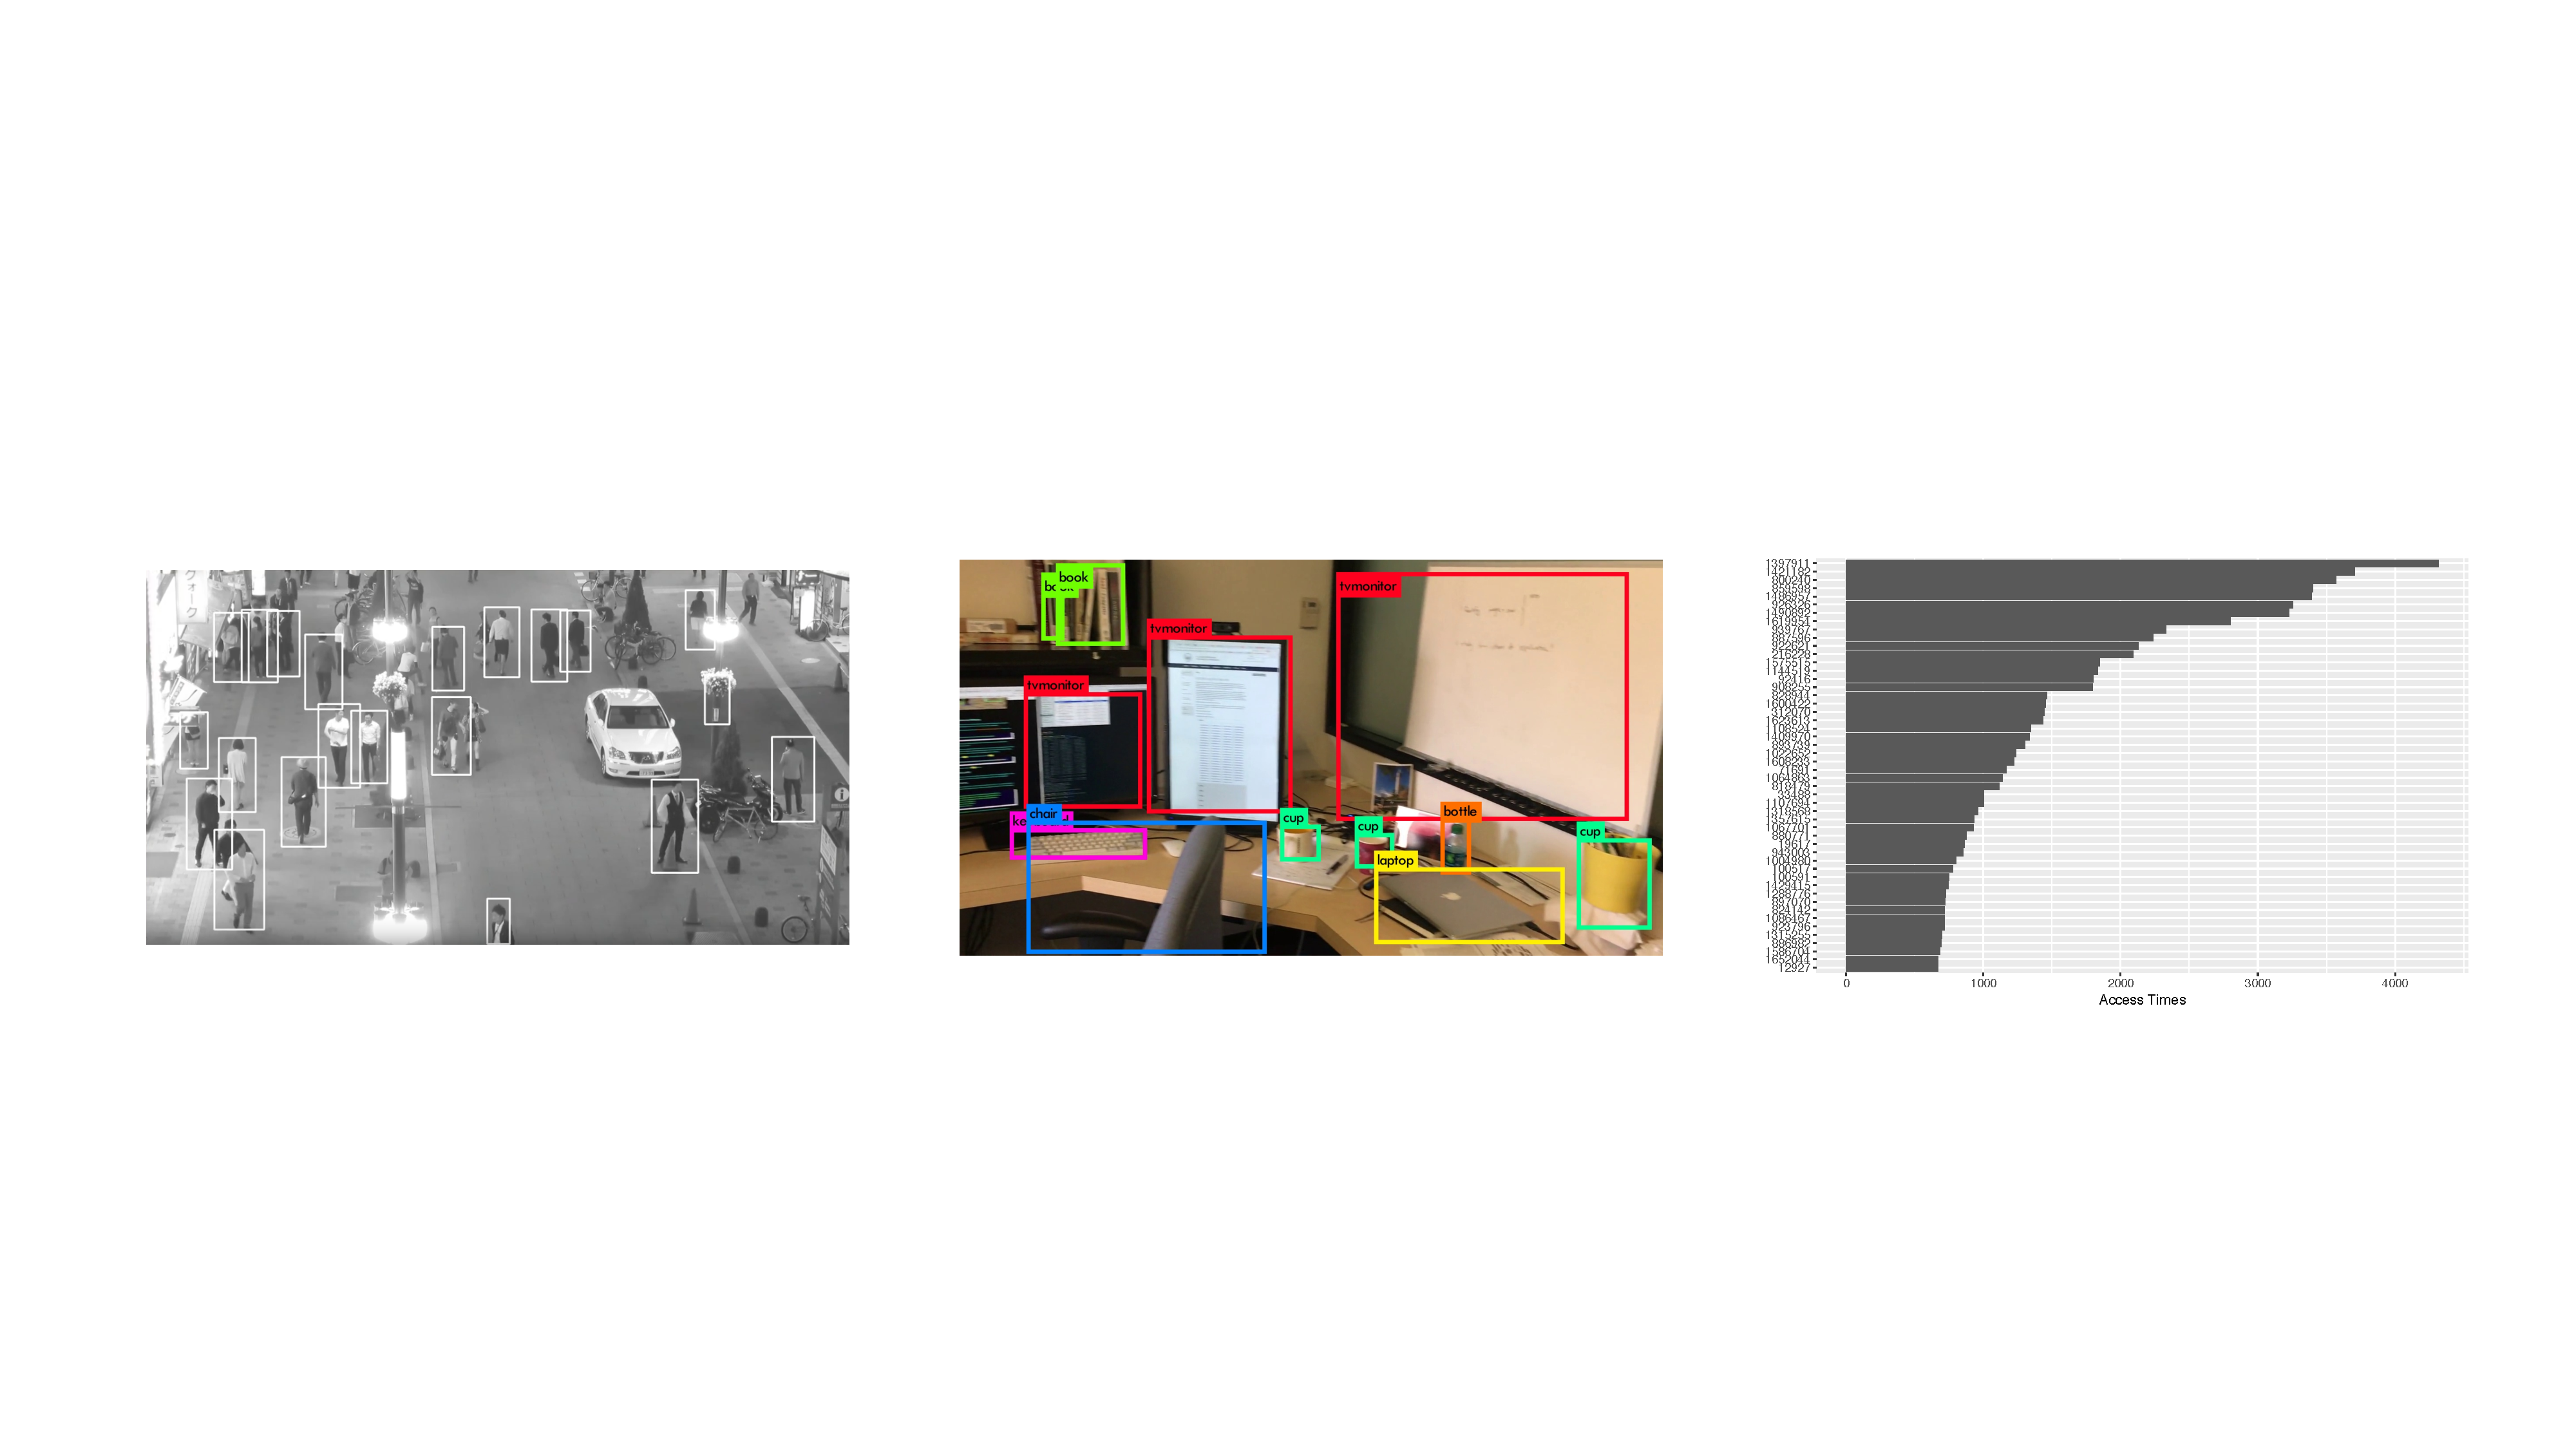
\includegraphics[width=.95\textwidth]{figures/apps.pdf}
  \caption{\sysname{} applications}
  \label{fig:apps}
\end{figure*}

\para{Pedestrian Detection:} This application analyzes video streams from
installed CCTV cameras and detect pedestrians inside. The detection result is a
list of bounding boxes representing pedestrian's relative location within the
view. Variant of this application can be used for safety monitoring, anomaly
detection or waiting line counting.

We implement most image-related operations using OpenCV
3.1~\cite{opencvlibrary}. The pedestrian detection uses histogram of oriented
gradients (HOG)~\cite{dalal2005histograms} with the default linear SVM
classifier. To ensure real-time processing of frames, GPU-accelerated
implementation is used in favor of the CPU-based implementation.

For video encoding, H.264 scheme is chosen for its prevalence in existing
systems. Our implemenation is based on GStreamer~\cite{gstreamer}, using
\texttt{x264enc} plugin. To integrate with \sysname{}, we create a pipeline that
exposes \texttt{appsrc} (to feed raw image data) and \texttt{appsink} (to get
encoded bytes). The GStreamer main loop is managed in a separate thread and
\sysname{} communicate with it via Rust's channel. The \texttt{x264enc} is
configured with \texttt{zerolatency} present and runs using four threads. It
uses constant quality encoding and the quantizer is exported as a parameter that
can be tuned.

This application has three degradation operations: reducing image resolution,
dropping frame rate or lower video encoding quality. We use F1 score as the
utility function. F1 score (\%) is the harmonic mean of precision and
recall~\cite{Rijsbergen:1979:IR:539927}. Here a successful detection is defined
when the intersection over union (IOU) is greater than
50\%~\cite{everingham2010pascal}.

\para{Augmented Reality:} We target at mobile augmented reality applications
which offload the heavy computation to resources elsewhere. Although local
computation is gaining attraction~\cite{satyanarayanan2009case, zhang2015cloud},
wireless communication link is also susceptible to capacity variation.

We use a similar setup as the pedestrian detection application except the actual
function that analyzes the stream. To recognize objects, we use a a pre-trained
neural network~\cite{darknet13} that's trained with
Imagenet~\cite{krizhevsky2012imagenet}. Similar to our first application,
GPU-accelerated implementation is use in favor for real-time processing.

The utility function here is more strict than the pedestrian detection:
true-positive depends not only on IOU criteria, but also on the type of objects
(a correct identification).

\para{Distributed Top-K:} Many distributed system monitoring applications
require to answer the ``top-k'' question~\cite{babcock2003distributed}, such as
the top-k most popular URLs or the top-k most access files. Naive methods of
transmitting all the raw log entries to the aggregation point is not feasible as
popular servers typically have millions of requests per second. Local worker
node can first perform a transformation that generates data summary, such as
key-value pairs of \texttt{<item, count>}. Even after this operation, the data
size could still be large given most real-world access patterns follow a
long-tailed distribution. There is a large-but-irrelevant tail that may be
unnecessary to send.

We consider two degradation operations: (1) a \texttt{head} operation that
performs a local Top-\texttt{N} first; (2) a local threshold \texttt{T} that
filters the tail. Obviously, these two operations are not orthognal to each
other. The impact on data size and quality depends on the distribution of the
actual data.

To evaluate the degradation impact, we use Kendall's W, which is a distance
measure of the concordance between two ranked list. The function outputs a
statistic measure ranging from 0 to 1, representing no agreement to complete
aggrement, respectively~\cite{abdi2007kendall}.

%%% Local Variables:
%%% mode: latex
%%% TeX-master: "sigcomm2017"
%%% End:
